\chapter{无人机编队整体控制逻辑、仿真环境以及硬件选型}
\label{chap:hardware}
本章主要介绍无人机编队的编队控制算法之外的系统组成部分;之后介绍无人机编队的整体的控制的实现逻辑,之后将介绍无人机编队的动力学仿真环境的搭建。
最后将介绍本次设计之中所用到的无人机型号,自动驾驶仪硬件以及姿态自动驾驶仪内环基本控制逻辑。
\section{无人机编队整体控制逻辑}
本文所设计的编队控制器是以开源自动驾驶仪内环为基础的,自动驾驶仪内环的作用是追踪来自位置环的无人机期望姿态;
算法所运行的软件环境是$ROS(Robot Operating System)$。$ROS$是一个适用于机器人的开源操作系统。它提供了操作系统应有的服务,包括硬件抽象,底层设备控制,常用函数实现,进程间消息传递,以及包管理。它也提供用于获取、编译、编写、和跨计算机运行代码所需的工具和库函数。本次使用的应用程序接口,正是$ROS$下的$mavros$功能包,本功能包的作用是:将来自自动驾驶仪的无人机状态数据由$mavlink$通信协议转换为$ROS$的进程间的通讯的协议;将来自编队控制器的姿态驾驶仪内环的期望姿态角以及期望油门值按照$mavlink$的协议进行编码,从而起到沟通编队控制器以及姿态驾驶仪内环的桥梁作用。软件层面的整体控制逻辑如下图所示:
\begin{figure}[H]
    \centering
    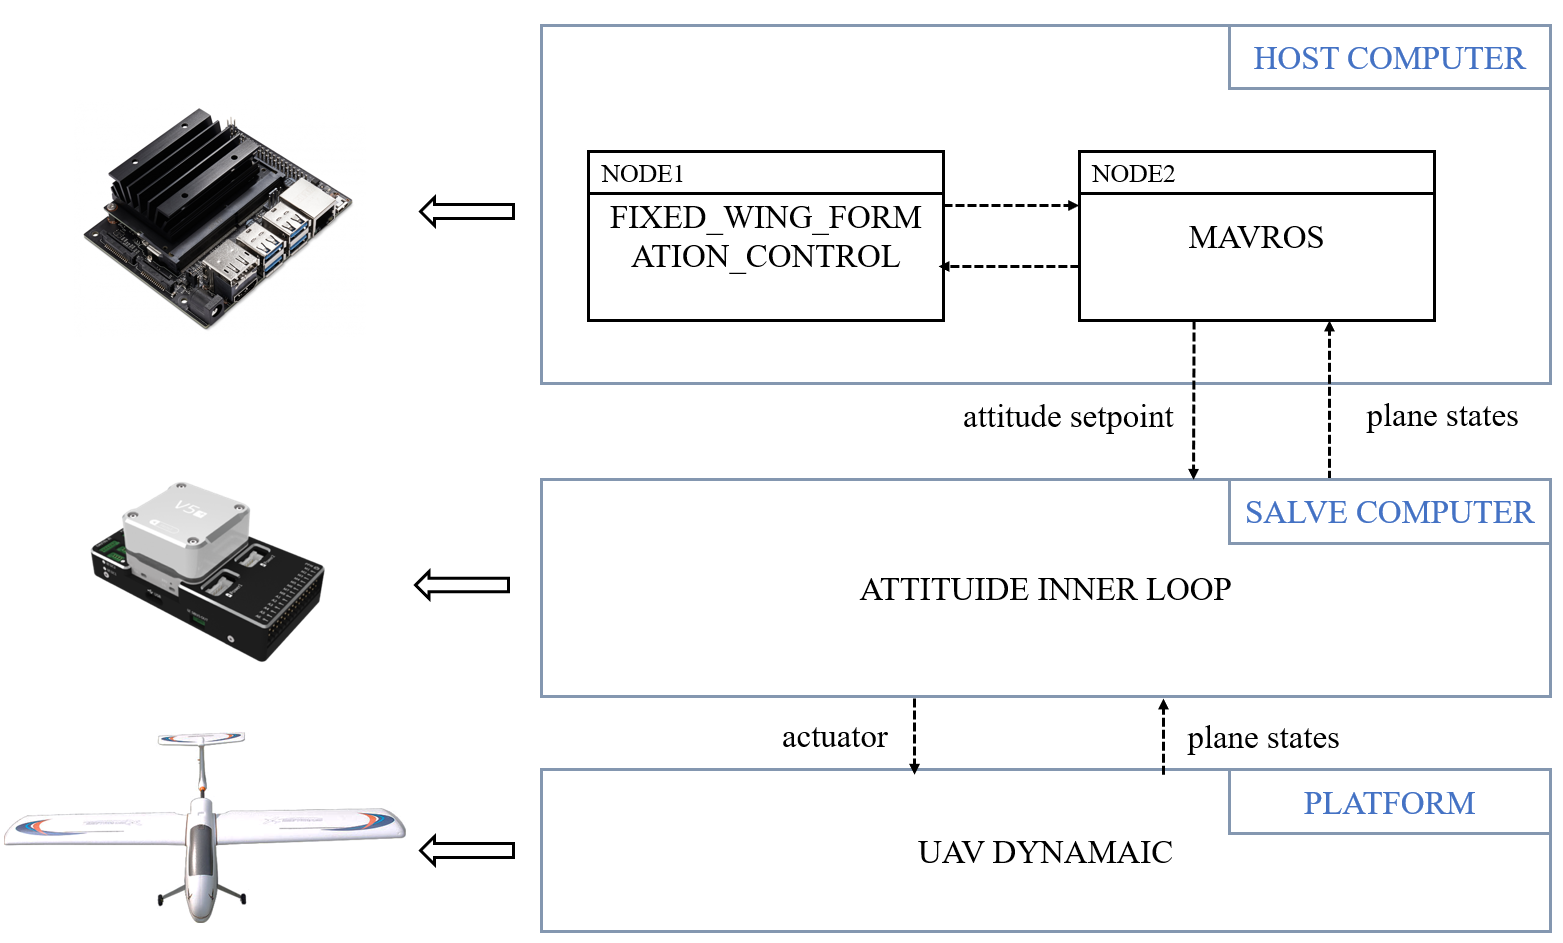
\includegraphics[width=1\textwidth]{figures/c4/c4-soft-hard.png}
    \caption{硬件软件选配关系}\label{fig:c4-soft-hard.png}
\end{figure}

\section{无人机编队仿真环境}
\section{无人机编队硬件选型}
本次毕业设计之中所涉及的编队控制器的自动驾驶仪部分为开源硬件$Pixhawk$:
